\chapter{Introduction}
\label{chapter1}

One of the greatest difficulties faced by patients with allergies or other food intolerances is the proper identification of which products they can safely consume. This task becomes much more complex when the patient is in a foreign country, where the products will usually be packaged in a language different from their mother tongue. At a time when the prevalence of food allergies continues to increase \cite{tang_food_2017}, as is the number of young Spaniards emigrating abroad \cite{dominguez-mujica_international_2018}, finding an effective solution to this problem has become ever more necessary.
    
In particular, in some countries like South Korea, the language barrier for foreign residents (who only constitute a mere 3.9\% of the total population \cite{noauthor__2021-1}) represents a hurdle hard to obviate.
    
The Korean language is classified by the US Foreign Service Institute as one of the 5 most difficult languages to learn for a native English speaker, requiring up to 2200 hours of study \cite{noauthor_foreign_2021}. Furthermore, in a study based on the domain acquired after 24 weeks of study, Chiswick and Miller assigned it the maximum lexical distance from English \cite{chiswick_linguistic_2005}.

One of the main factors contributing to this difference is that Korean uses their own native alphabet, \textit{hangeul}, composed of 24 basic characters that are combined to form syllabic blocks \cite{noauthor_hangul_2021}. The Figure \ref{fig:label} depicts a real example of text in \textit{hangeul}.

\begin{figure}[h]
  \centering
  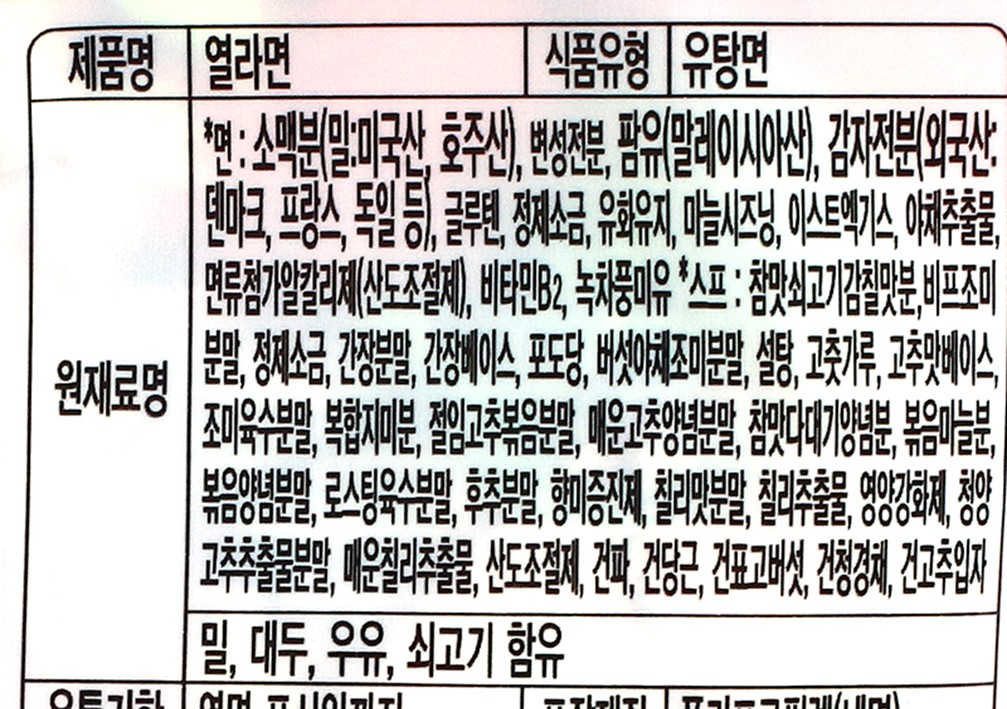
\includegraphics[width=0.5\textwidth]{Figures/label.jpg}
  \caption{%
    Label of a packaged food product in Korean
  }
  \label{fig:label}
\end{figure}

The barrier across these languages that make use of different alphabets or scripts makes basic tasks such as the input of text in a translator laborious to those who may not be familiar with the appropriate tools (Korean keyboards, OCR systems, speech-to-text, etc.). These methods, like the most commonly used shown in Figure \ref{fig:keyboard}, often require the user to have an entry-level knowledge of Korean language in general or \textit{hangeul} in particular, which may take some time to acquire for newcomers to South Korea.

\begin{figure}[h]
    \begin{subfigure}{0.5\textwidth}
        \centering
        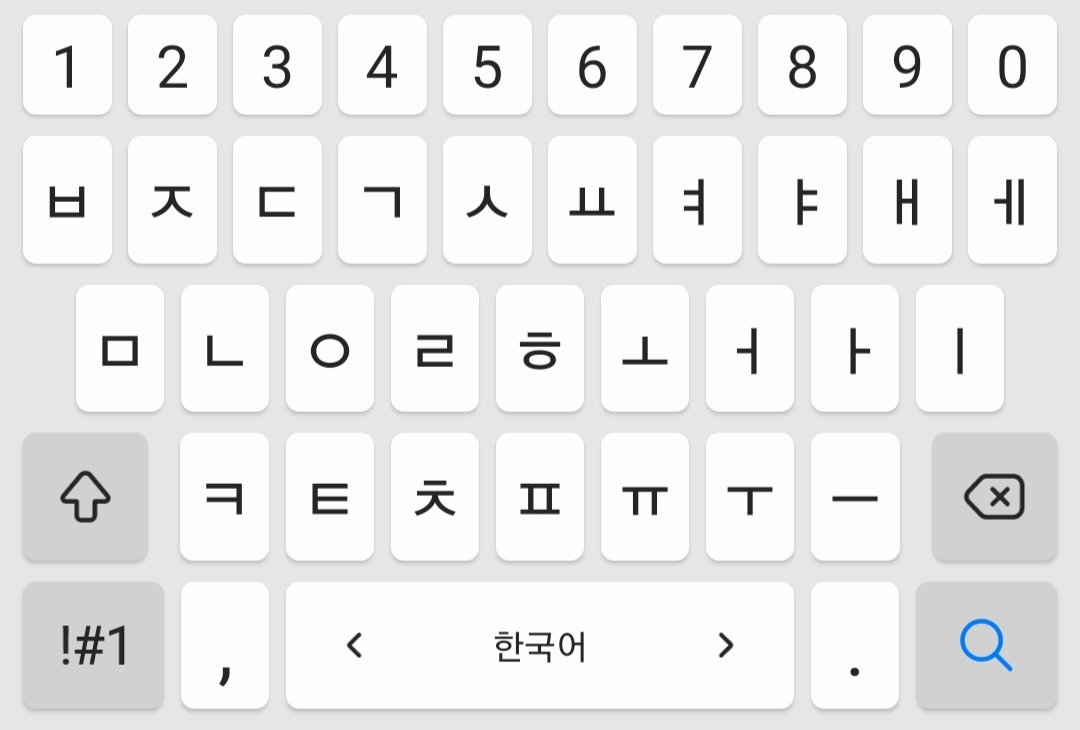
\includegraphics[width=0.9\linewidth]{Figures/2beolsik.jpg} 
        \caption{2-beolsik}
        \label{fig:2beolsik}
    \end{subfigure}
    \begin{subfigure}{0.5\textwidth}
        \centering
        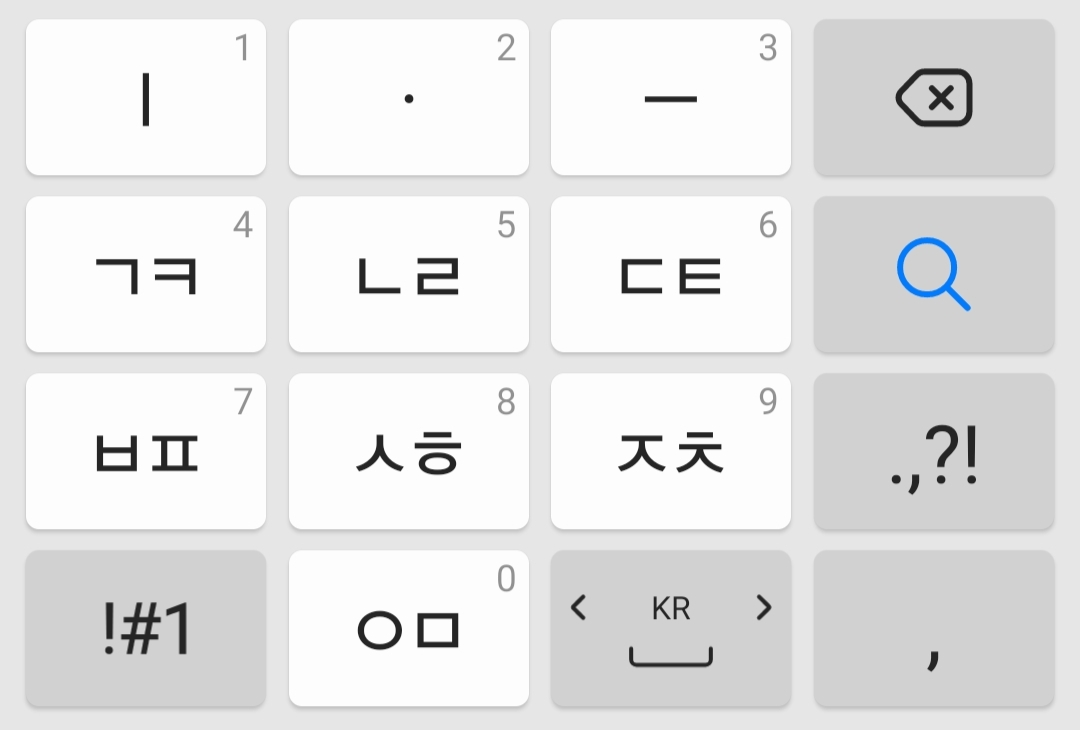
\includegraphics[width=0.9\linewidth]{Figures/chunjiin.jpg}
        \caption{Chunjiin}
        \label{fig:chunjiin}
    \end{subfigure}
    \caption{Korean keyboard layouts}
    \label{fig:keyboard}
\end{figure}

This combination of factors complicate such an elementary and vital process for an allergy patient as is understanding the labeling of a product, reading its ingredients and identifying what possible allergens it may include.

\section{Motivation}
    
To assist in this task, this Degree Final Project (DFP) will focus on producing a mobile application whose main functionality allows scanning the text in the list of ingredients for any packaged food product. Based on the substances specified by the user, the application will issue a warning if any of them are found among the recognized words.
    
This idea is mainly motivated by the experience of the author, who currently resides in South Korea, as well as by the experiences of his acquaintances with allergies and of all those to whom its use is extended: vegetarians, vegans, celiacs, lactose intolerant, consumers of halal products, \textit{kosher} products, etc. Likewise, this concept could potentially be ported to support other languages and scripts, thus increasing the target audience to every foreign person having difficulties reading labels written in language of the country where they reside.

Another relevant reason for choosing this topic for the DFP was that it represents a great opportunity to bridge the knowledge acquired through some of the courses in the degree, such as mobile app development in \textit{Lines of Software Products}, UI design principles in \textit{User Interface Development} and database design in \textit{Databases}; with the fields studied during the stay in South Korea in courses like \textit{Image Processing}, \textit{Software Design} or \textit{Natural Language Processing}.

\section{Goals and scope}

The main intent to be achieved through the completion of this DFP, as it has been briefly detailed before, is the development of a mobile application that assists any person when discerning whether a certain product labeled in Korean contains any unwanted ingredient or allergen.

In the solution proposed in this thesis, the user should input manually in the app the list of undesired substances and products that must be detected on the food labels. Then, the user may take a picture of the ingredients list with the app and, depending on those substances specified before, the application will issue a warning if any matches are found between the recognized terms and the user blacklist.

To achieve the desired results, one the main challenges is performing an accurate OCR that allows scanning the list of ingredients in Korean for any packaged food product. As APIs that offer this kind of services for \textit{hangeul} script are usually paid or very limited, it is necessary to find a solution that allows for on-device, offline processing with a reasonable accuracy. An example of said text recognition systems in use can be seen in Figure \ref{fig:maplestory}, where the OCR Engine Tesseract \cite{noauthor_tesseract_2021} is applied to a popular Korean online game.

\begin{figure}[h]
  \centering
  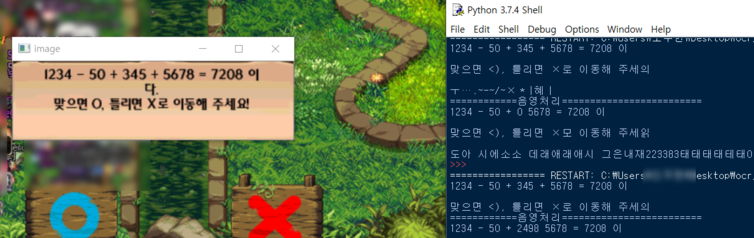
\includegraphics[width=\textwidth]{Figures/maplestory.png}
  \caption{%
    Example of an OCR engine reading \textit{hangeul} text
  }
  \label{fig:maplestory}
\end{figure}

Besides, this app aims to fulfill a niche as a cross-language ingredient scanner. The most popular commercial applications that already scan products and provide nutritional information, such as \textit{Yuka} \cite{noauthor_yuka_nodate-1} or \textit{MyRealFood} \cite{sl_myrealfood_nodate}, often do not provide the detailed ingredients list and most importantly, will not recognize products sold outside of their target region. They are also oriented towards providing nutritional scores based on food additives and cater to an audience interested in the \textit{real food}\footnote{Denomination given to foods that are not manufactured by processing and that do not contain food additives.} lifestyle, rather than being suited for people dealing with food intolerances.

On the other hand, while translators can perform accurately when reading Latin script, they often underperform when needing to recognize \textit{hangeul} script or when facing lists with complex terms instead of more structured text. As such, the most fundamental goal of the app is to be able to provide accurate readings of ingredients in Korean language and present the information and alerts to the user in a clean and streamlined manner.

\section{Objectives}

The prime objective of this DFP is the production of a fully functional mobile app, which will require the implementation and coordination of an ensemble of existing technologies, techniques and frameworks.

In order to compose said application, the following subobjectives will need to be materialized:

\begin{itemize}
\item Collection and study of prior bibliography, analysis of the existing solutions and approaches to similar problems implemented by other authors and identification of any potential new requirements.
\item Selection and installation of the technologies and tools that will be needed through the development process, formation in said technologies.
\item Recognition of the text on the product label. From a photograph, usage of any sort of preprocessing \cite{noauthor_optical_2021} and character recognition \cite{islam_survey_2016} tools and techniques needed to obtain the raw text.
\item Analysis of the output text, identifying the different ingredients, implementing any post-processing methods if needed (tokenization, segmentation, dictionary correction, etc.) \cite{kargin_nlp_2021} and matching with database.
\item Translation of the output text to be used as a fallback resource for unrecognized terms, implementing both on-device translation as well as a translation service API.
\item Finding an adequate data source and construction of a database architecture that stores the set of ingredients and possible synonyms to detect for each user profile or dietary need.
\item Development of the frontend of the application with a simple and usable interface intended for Android mobile devices. The application will allow the user to enter the unwanted ingredients, capture the images of the packaging and will return the list of ingredients in English along with an alert if it detects any specified allergens.
\end{itemize}

The proposed architecture for the mobile application, upon completion of this objectives and accounting with the technologies finally chosen, is the one shown in Figure \ref{fig:architecture}.

\begin{figure}[h]
  \centering
  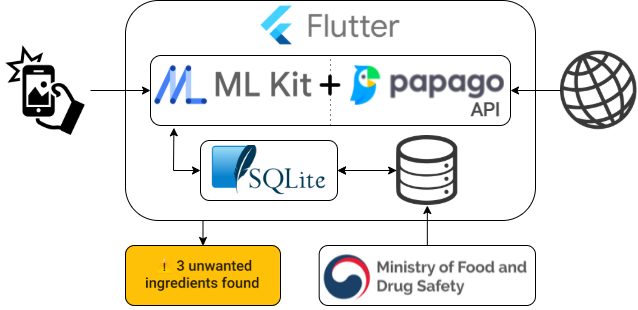
\includegraphics[width=\textwidth]{Figures/architecture.png}
  \caption{%
    Architecture of the mobile application
  }
  \label{fig:architecture}
\end{figure}

\section{Structure of this thesis}

In Chapter \ref{chapter1} we have introduced the main idea of our project, providing the adequate context to motivate and justify the topic for this thesis, as well as outlining the main goals and objectives that are expected to be met during its development.

Chapter \ref{chapter2} presents a compilation of previous works that tackle the same problem taken from the literature as well as including some commercial applications.

Through Chapter \ref{chapter3}, the planned schedule for the project is presented, defining in more detail the different tasks and subtasks that have been completed using a Gantt diagram. The time distribution is also discussed, justifying the varying amount of work hours allocated to each different task.

After it, Chapter \ref{chapter4} describes the software development methodology used through the work, presenting any relevant workflows or organization techniques used through the process.

The tools and technologies utilized for the completion of this project are detailed in Chapter \ref{chapter5}, providing a description about each of them and justifying the choice above other similar solutions.

Chapter \ref{chapter6} goes in detail through the whole development process, explaining every step of the implementation and reporting every problem encountered as well as the solutions that were found to overcome them.

In Chapter \ref{chapter7}, the results of the project are shown through practical examples and use cases to test the application behaviour and accuracy.

Finally, Chapter \ref{chapter8} presents the conclusions and lessons learned after the completion of the project, as well as introducing some other potential ideas for further iterations of the mobile application.